\section{Conformal Invariance}
\label{ch:conf}

\begin{figure}[b]
\begin{center}
    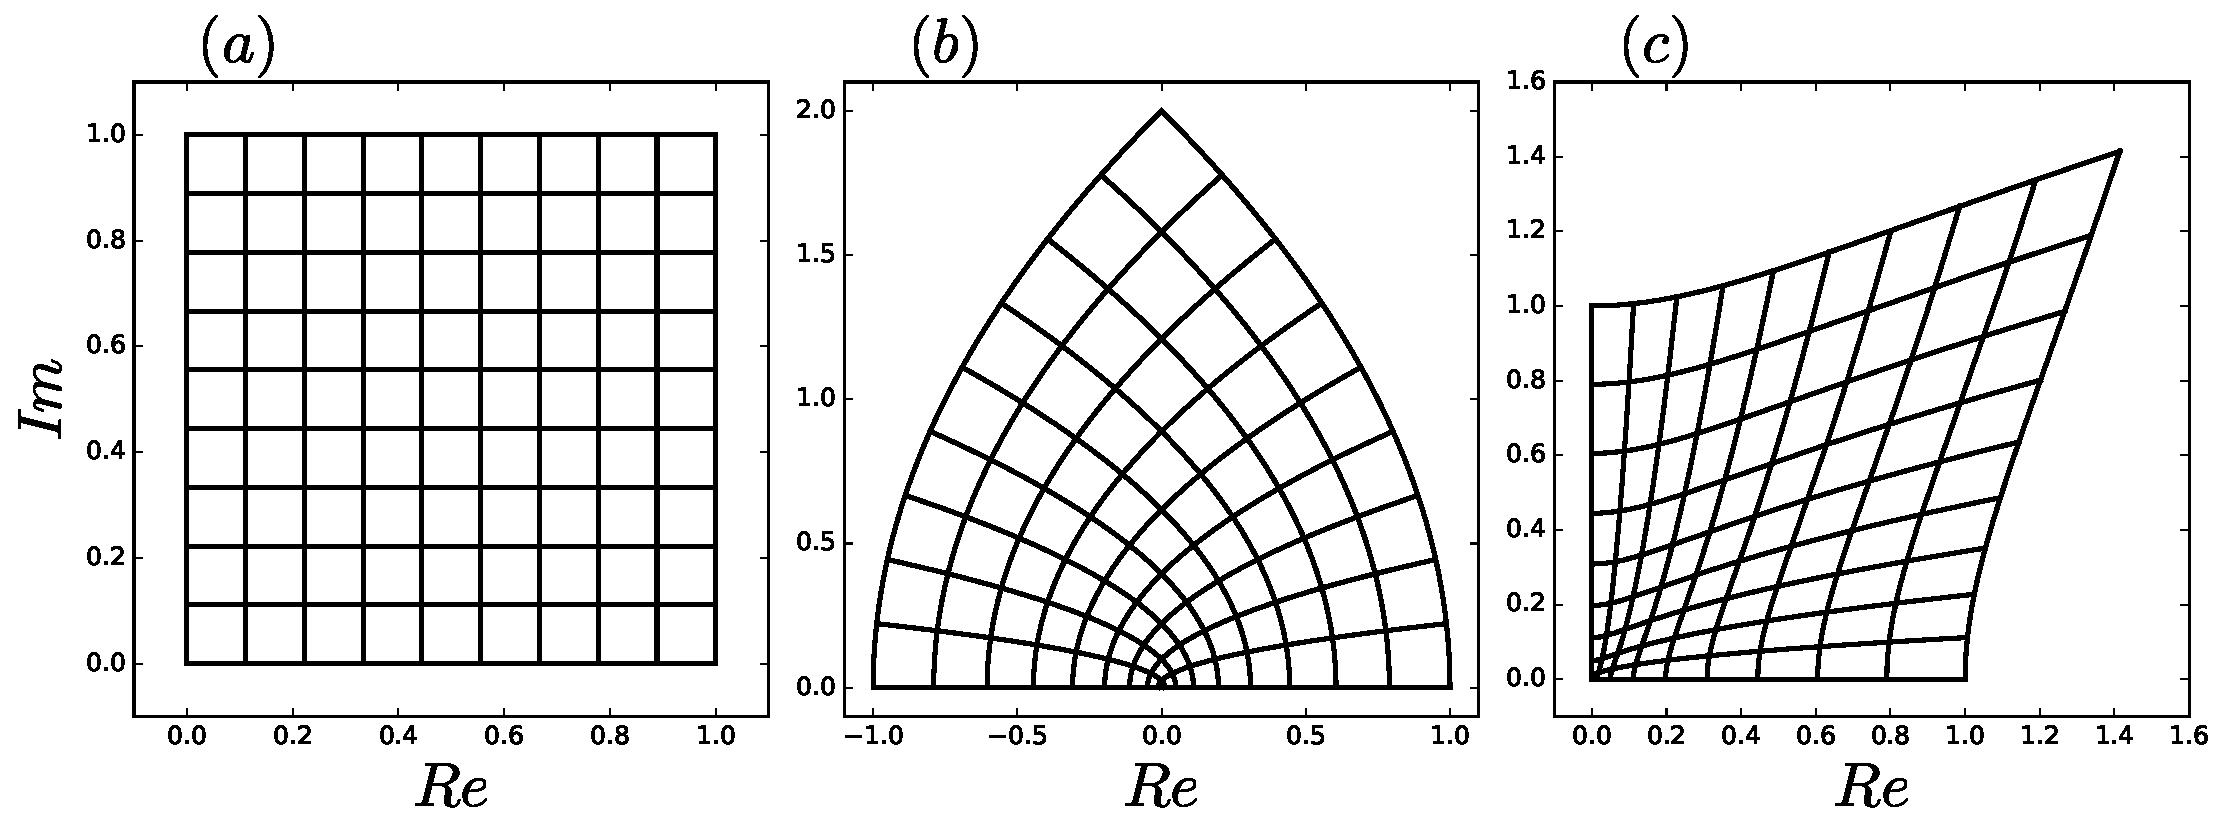
\includegraphics[width=0.9\textwidth]{chapters/ch3-conf/figs/cmapex}
\end{center}
\caption{Coordinates transformations in the complex plane can be divided into
    conformal and non-conformal. Conformal transformations preserve the
    intersection angles between lines, unlike the non-conformal. The
    transformation from the square lattice in (a) into (b) is conformal
    ($f(z)=z^2$), while the one from (a) to (c) ($f(z)=z|z|$) is not.}
\label{fig:cmapex}
\end{figure}

In Section~\ref{sec:scaling} we talked about the principle of scale invariance
and how incredibly useful it is. It is based on the fact that the correlation
functions transform covariantly under a change in scale $\mathbf{r}\rightarrow
b\mathbf{r}$. A \textit{global} change in scale, that is. One could imagine a
transformation $\mathbf{r}\rightarrow f(\mathbf{r})$ in which the scaling
factor $b$ depends on the position. This would be a \textit{local} change of
scale. This kind of transformation would deform the overall shape of the
system, but in the direct vicinity of a point it would look like a regular
scale transformation with possibly a rotation and translation. Surely we don't
expect every possible functional form of $f$ to behave like that, some of them would
deform the geometry of the system even at the very small scales, so we must be
careful when trying to generalize scale invariance. Luckily there is a class of
functions that look like exactly what we want, these are called
\textit{conformal transformations} or \textit{conformal maps}.

A transformation $\mathbf{r}\rightarrow\mathbf{r}'$ is conformal when it
preserve the angle between any two vectors, that is
\begin{equation}
    \theta=
    \arccos\frac{\mathbf{r}_{1}\cdot\mathbf{r}_{2}}
                {\left|\mathbf{r}_{1}\right|\left|\mathbf{r}_{2}\right|}=
    \arccos\frac{\mathbf{r}'_{1}\cdot\mathbf{r}'_{2}}
                {\left|\mathbf{r}'_{1}\right|\left|\mathbf{r}'_{2}\right|}=
    \theta',
\end{equation}
as illustrated in Figure~\ref{fig:cmapex}. More formally, they are coordinate
changes that that keep the metric invariant up to a local scaling factor
\begin{equation}
    g_{\mu\nu}'\left(\mathbf{r}'\right)=
    \Omega\left(\mathbf{r}\right)g_{\mu\nu}\left(\mathbf{r}\right).
\end{equation}
Figure~\ref{fig:lenna} shows an example of the same conformal map being applied
to a large and a small image, showing how it does not deform the latter, it can
only scale, translate or rotate it. Because of that, translational, rotational,
and scaling invariance are obvious properties a system must have in order to be
conformally invariant. Another important ingredient is locality, that is, the
presence of short range interactions. That's because if different parts of the
system will be rescaled by different factors, they must not exert direct
influence over one another (they can exert \textit{indirect} influence through
long range correlations though). The recipe for conformal invariance is, as
Cardy~\cite{Domb1972} puts it
\begin{equation*}
    \left.
        \begin{array}{l}
            \mbox{Scale Invariance}\\
            \begin{array}{cl}
                + & \mbox{Translation Invariance}\\
                + & \mbox{Rotational Invariance}\\
                + & \mbox{Short-range Interactions}
            \end{array}
        \end{array}
    \right\} \Rightarrow\mbox{Conformal Invariance}.
\end{equation*}
If any of these criteria is not met, conformal invariance breaks down, which is
the case of non-local models like minimum spanning trees (given a fully
connected graph with randomly weighted edges, the minimum spanning tree is a
loopless sub-graph that connects all vertices while minimizing the sum of the
weights)~\cite{Wilson2004}, or even anisotropic systems as described in
Section~\ref{ch:anis}.

We can implement the idea of conformal invariance in a similar way we did
for scale invariance in Eqs.~\ref{eq:scal} and~\ref{eq:scal10}.
This way, the $n$-point correlation function of any set of field
operators $\{\phi_i\}$ transforms as follows
\begin{equation}
    \label{eq:cinv}
    \left\langle
        \phi_{1}\left(\mathbf{r}_{1}\right)
        \phi_{2}\left(\mathbf{r}_{2}\right)
        \cdots
        \phi_{N}\left(\mathbf{r}_{N}\right)
    \right\rangle =
    \prod_{i=1}^{N}J{\left(\mathbf{r}_{i}\right)}^{-x_{i}}
    \left\langle
        \phi_{1}\left(\mathbf{r}_{1}'\right)
        \phi_{2}\left(\mathbf{r}_{2}'\right)
        \cdots
        \phi_{N}\left(\mathbf{r}_{N}'\right)
    \right\rangle,
\end{equation}
where in this case $J$ stands for the Jacobian of the transformation
$J{\left(\mathbf{r}\right)}^{d}=
\det\left(\partial\mathbf{r}/\partial\mathbf{r}'\right)$, and the $x_i$ are the
scaling dimension of each operator. Figure~\ref{fig:isingcm} shows how the Ising
model in the critical (conformally invariant) point behave under a conformal
transformation. Despite being deformed, the cluster structure remains
statistically similar, while above the critical point, which is not conformally
invariant, the cluster structure is clearly non uniform after a deformation, as
shown in Figure~\ref{fig:isingcm2}.

\begin{figure}
\begin{center}
    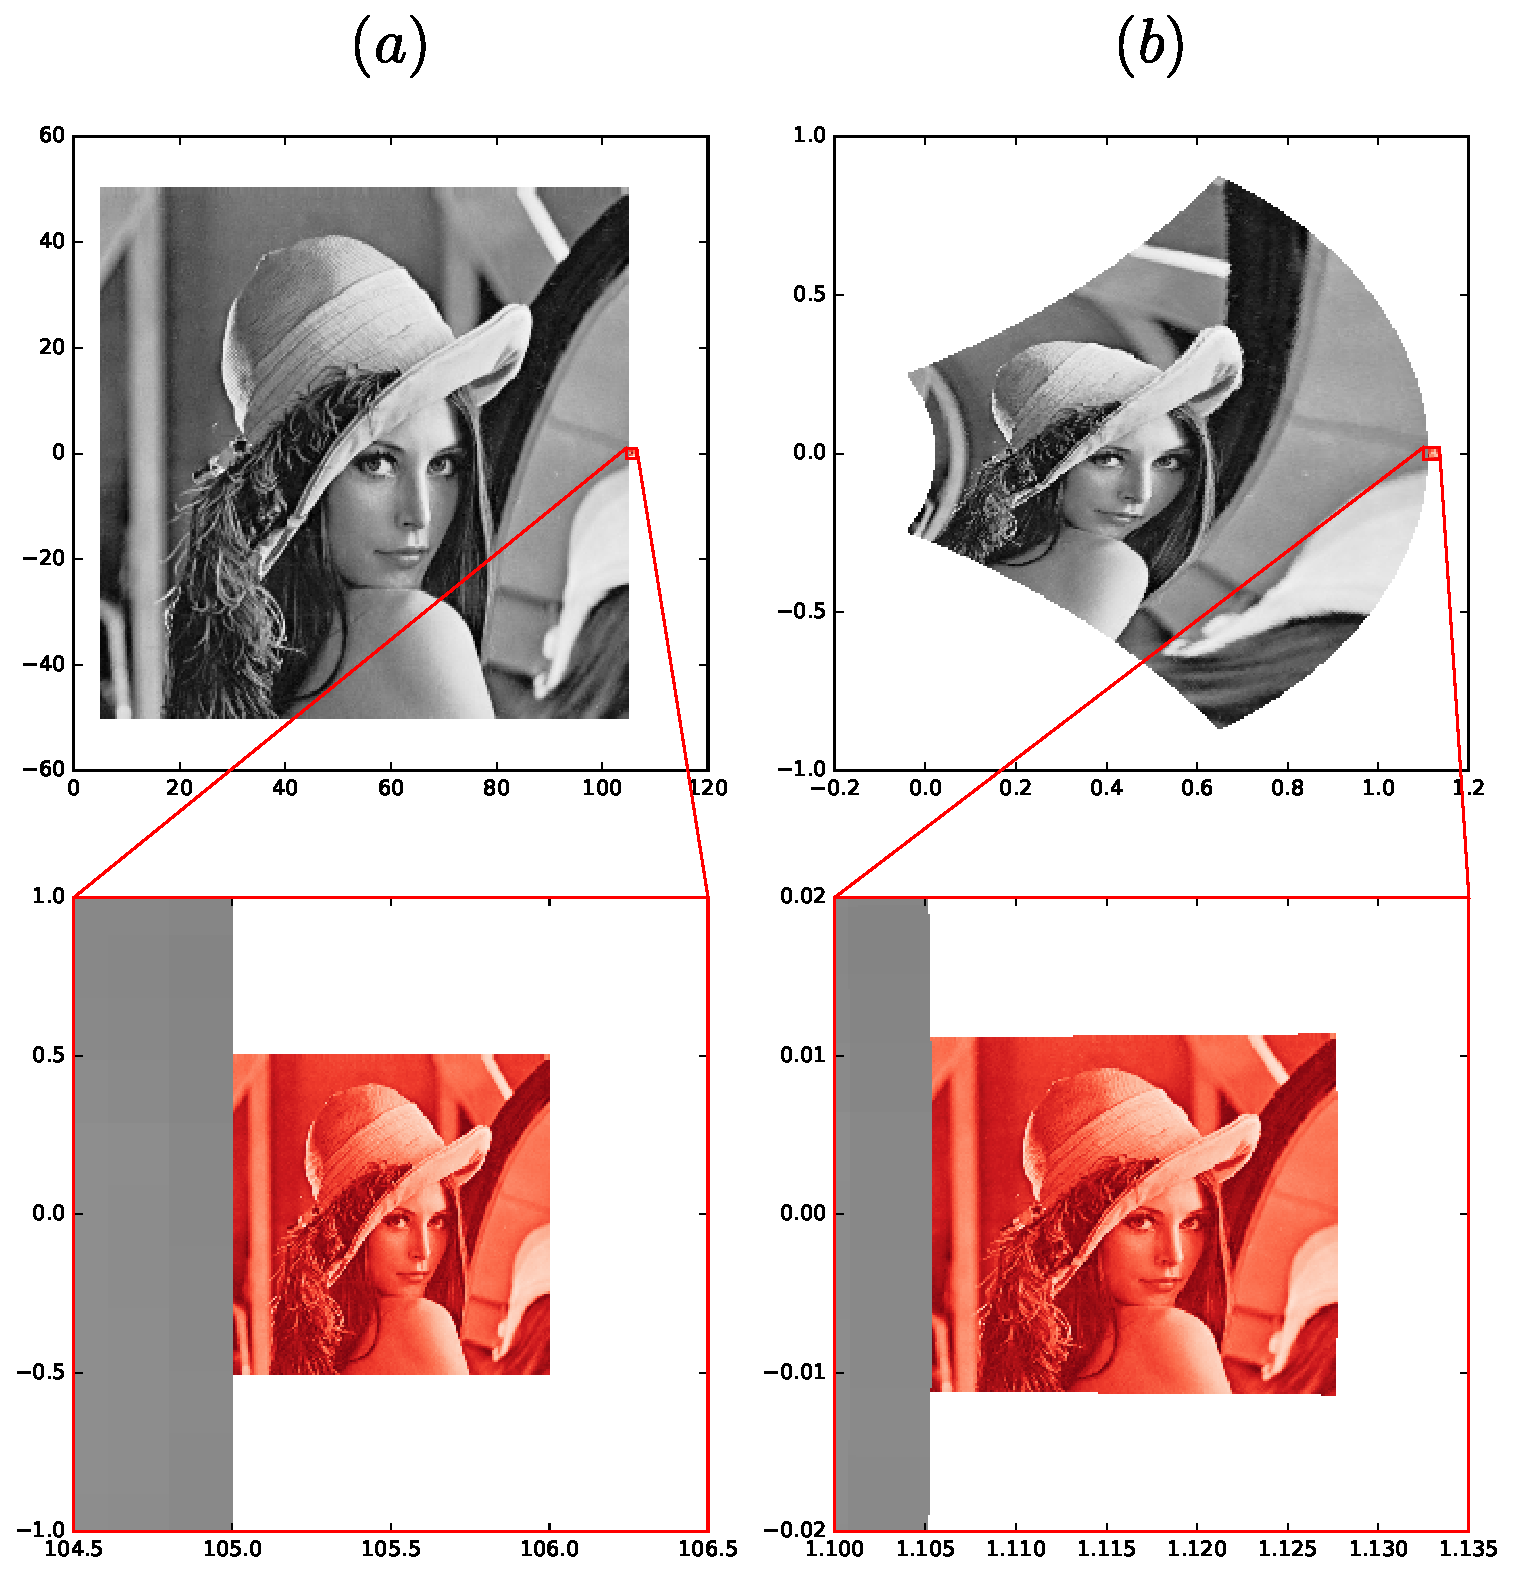
\includegraphics[width=0.66\textwidth]{chapters/ch3-conf/figs/lenna}
\end{center}
\caption{Two identical images, one large (in grayscale) and the other small (in
    red, shown in the zoom), are transformed from (a) to (b) using a conformal
    map $f(z)=z/(200-z)$. While the large one is heavily deformed, the smaller
    one was only translated and shrunk. This illustrates the fact that conformal
    maps behave locally as a scale transformation.}
\label{fig:lenna}
\end{figure}


In $d>2$ the group of conformal transformations is finite dimensional, and
it is composed of only translations, rotations, dilations and the special
transformation
\begin{equation}
    \mathbf{r}\rightarrow\mathbf{r}'=
    \frac{\mathbf{r}+\mathbf{a}r^{2}}{1+2\mathbf{a}\cdot\mathbf{r}+a^{2}r^{2}}.
\end{equation}
These maps are known as projective conformal transformations, and are capable
of completely determining 2-point and 3-point correlation functions. Higher
order correlators, however, cannot be determined using conformal invariance.
Determining these correlators are important in determining the critical
exponents through field theoretical series expansions~\cite{Henkel2013}.

In $d=2$, however, the conformal group is infinite dimensional and homeomorphic
to the set of analytical functions. This makes conformal invariance an
incredibly powerful tool to analyze and characterize conformal field theories
in two dimensions, since more symmetries implies more constraints over the
behavior of the system.

Since the mathematics of analytical functions live and thrive in the complex
plane, it is common to shift the analysis to it by making the transformations
\begin{equation}
    \begin{array}{cc}
        z=x+iy, & \bar{z}=x-iy
    \end{array}
\end{equation}
This way, all projective transformations can be condensed into one functional
form
\begin{equation}
    w\left(z\right)=\frac{az+b}{cz+d},\;\;\;\;\;\;\;\; ad-bc=1.
\end{equation}
Operators that transform according to Eq.~\ref{eq:cinv} when subject to
projective transformations are called quasi-primary operators.
As mentioned before, the two-point correlation function is fixed and given by
\begin{equation}
    \label{eq:twop}
    \left\langle
        \phi_{1}\left(z_{1}\right)\phi_{2}\left(z_{2}\right)
    \right\rangle =
    \frac{1}{\left|z_{1}-z_{2}\right|^{2(h_{1}+h_{2})}}.
\end{equation}
Where $h_{1,2}$ are called the conformal weights. This relation is consistent
with Eq.~\ref{eq:critcor} and indicates that $\eta=4h$ when $h_1=h_2$.

Fields covariant under any conformal map are called primary operators. The
magnetization density and energy density fields of the ising model are primary
operators, for example. We can derive an important result of critical phenomena
by looking at how primary operators transform under the map
$f(z)=L\log(z)/2\pi$, which maps the whole plane to an infinite strip of length
$L$. Applying it to Eqs.~\ref{eq:cinv} and~\ref{eq:twop} we get a relation
between the scaling dimension $x$ of the operator, correlation length $\xi$ and
system size $L$
\begin{equation}
    \xi=\frac{L}{2\pi x}.
\end{equation}
Therefore, conformal invariance produced a prediction of the finite-size
scaling of the correlation length on a finite system.

A particularly important quasi-primary operator is the stress-energy tensor,
related to the ``stiffness'' of the action when the system is subject to a small
deformation $\mathbf{r}\rightarrow \mathbf{r} + \epsilon(\mathbf{r})$, which
should transform like
\begin{equation}
    \delta S=
    -\frac{1}{2\pi}
    \int d^{2}r\partial^{\mu}\epsilon T_{\mu\nu}\left(\mathbf{r}\right).
\end{equation}
Although it is a rank-2 tensor, it has ony one degree of freedom, namely
$T=(T_{11}-T_{22}-2iT_{12})/4$, which can be described by the expansion.
\begin{equation}
    T\left(w\right)T\left(z\right)=
    \frac{c}{2{\left(w-z\right)}^{4}}+
    \frac{2}{{\left(w-z\right)}^{2}}T\left(z\right)+
    \frac{1}{w-z}\partial T\left(z\right)+\mbox{regular}
\end{equation}
If $T$ were a primary operator the first term would no exist. So the constant
$c$ called the \textit{central charge}, measures how ``non-primary'' the stress
tensor is. A specific conformal field theory (and as a consequence, the model
being studied) is characterized by its central charge. The ising model, for
example, has $c=1/2$ and the 3-state Potts model has
$c=4/5$~\cite{Francesco1997}.

\begin{figure}
\begin{center}
    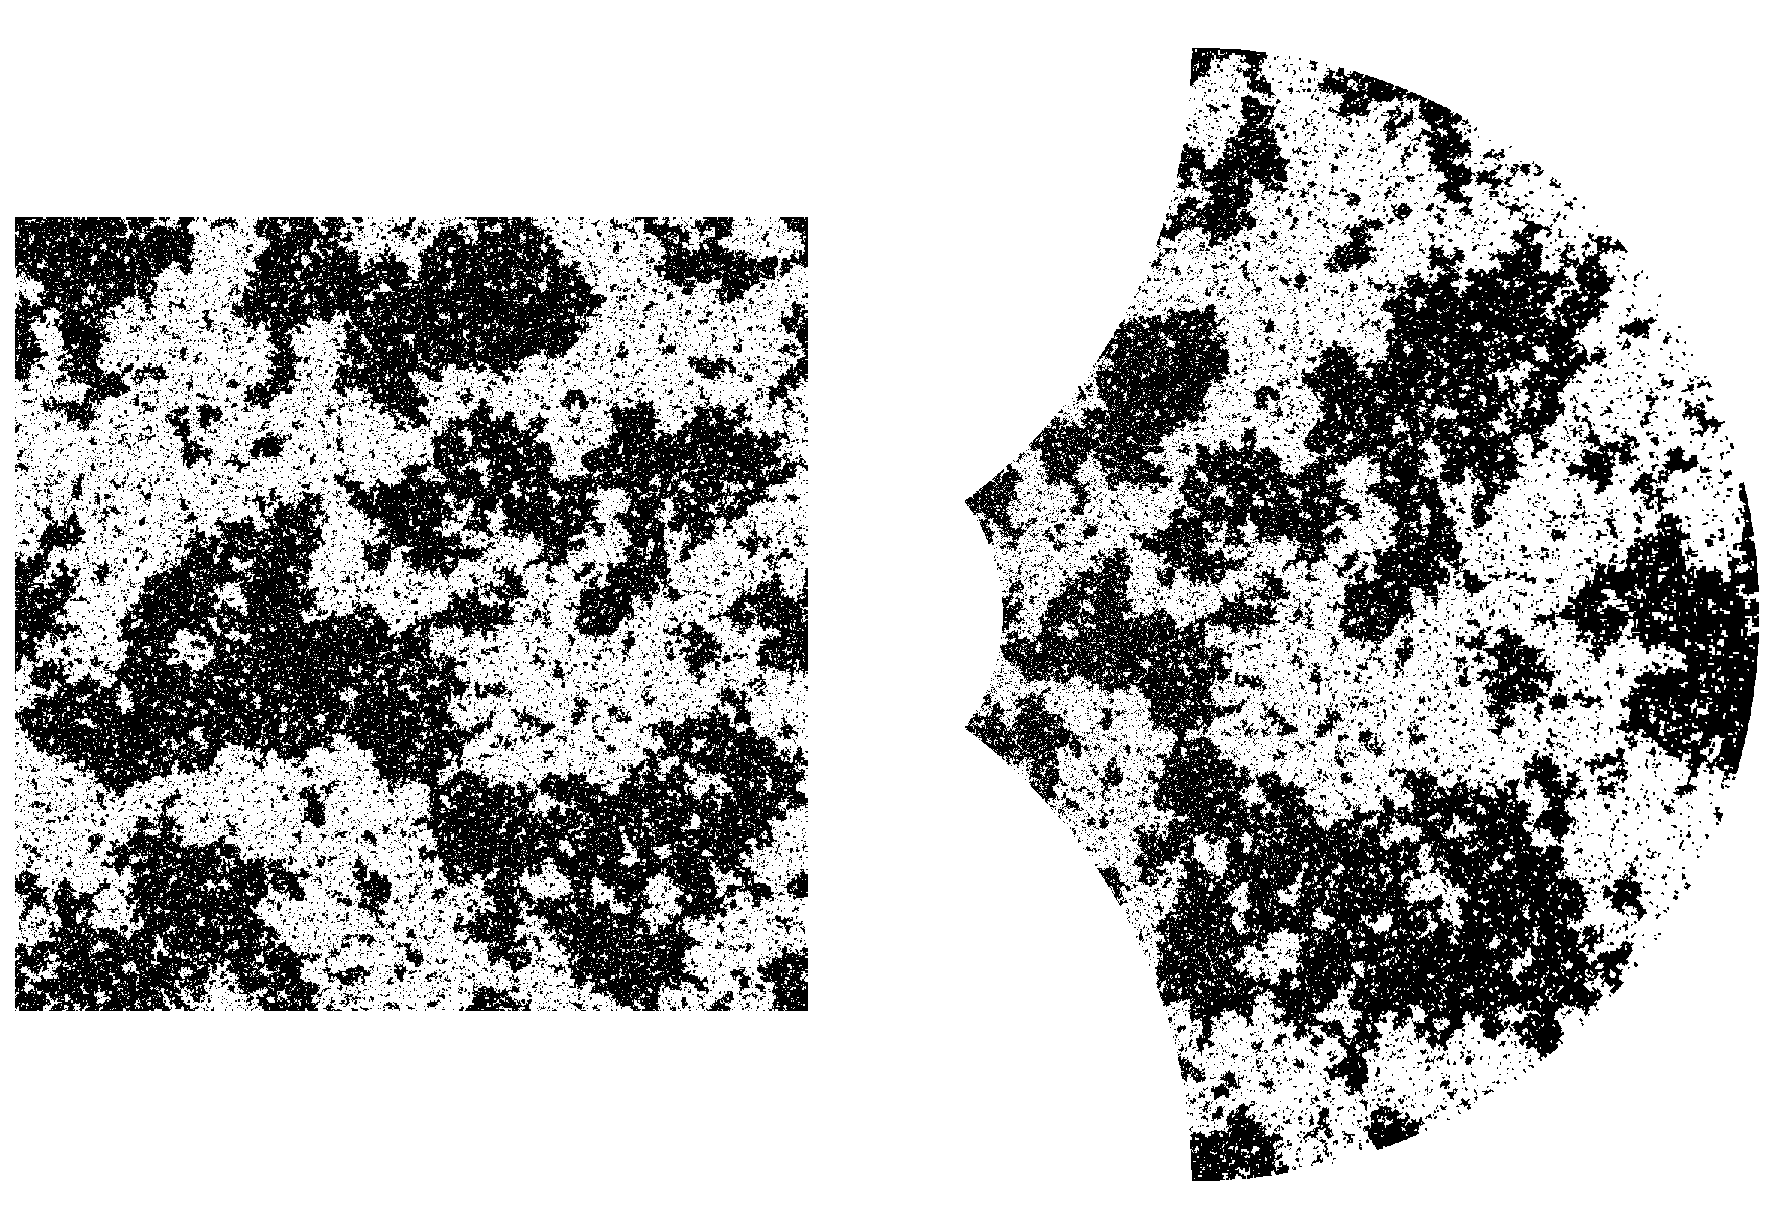
\includegraphics[width=0.8\textwidth]{chapters/ch3-conf/figs/isingcm}
\end{center}
\caption{Illustration of the Ising model at the critical point when transformed
    under a conformal map $f(z)=z/(2-z)$. The deformed image still looks
    statistically similar to the original, which is a consequence of conformal
    invariance.}
\label{fig:isingcm}
\end{figure}

\begin{figure}
\begin{center}
    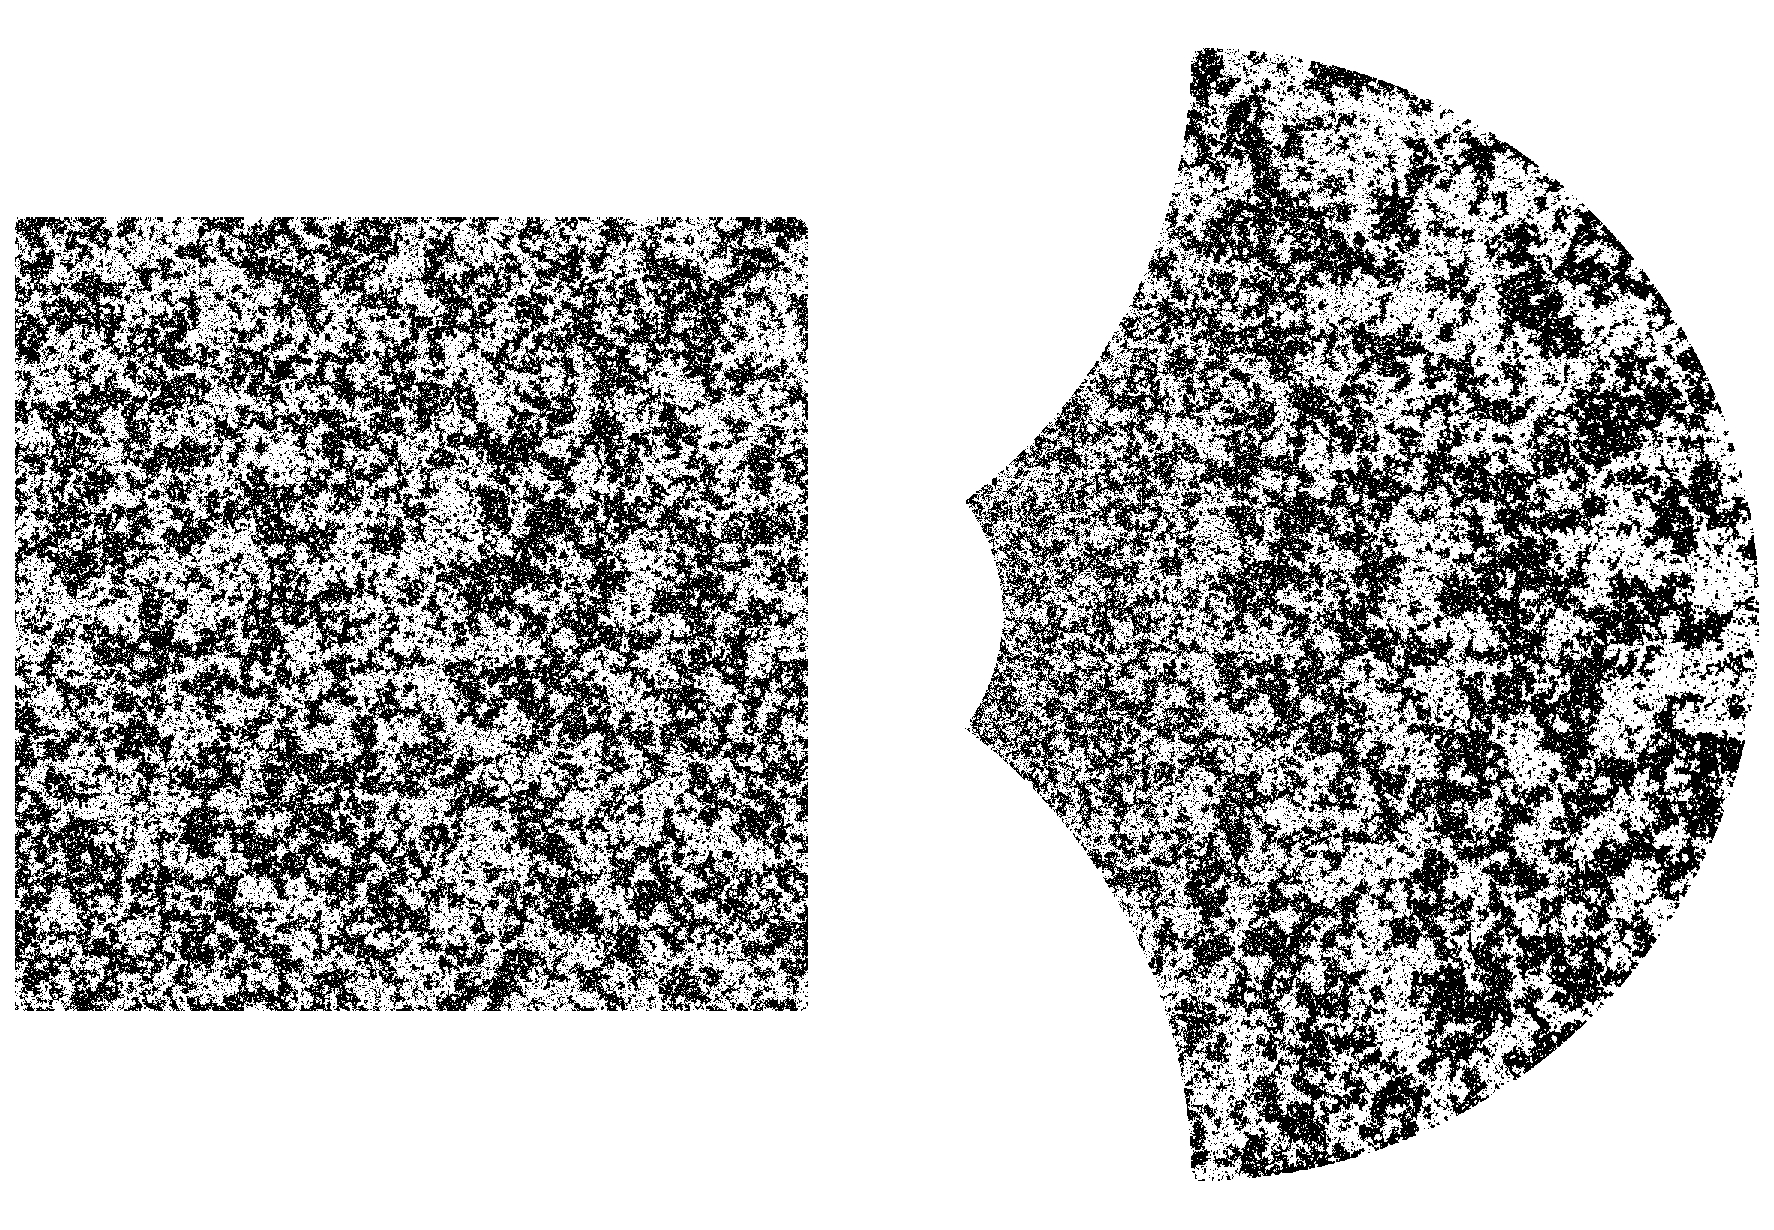
\includegraphics[width=0.8\textwidth]{chapters/ch3-conf/figs/isingcm2}
\end{center}
\caption{Illustration of the Ising model above the critical point when
    transformed under a conformal map $f(z)=z/(2-z)$. In the deformed image,
    the spin configuration is no longer homogeneous, because outside the
    critical point the system is no longer conformally invariant.}
\label{fig:isingcm2}
\end{figure}
